
Action Geometry is a method of geometric construction which uses sets of
standard shapes and constructions designed to physically replicate
themselves using practical physical media. We can make these shapes from
acrylic, plastics of all kinds, thin cardboard, thick cardboard, wood,
paper or stone. We design constructions which can be replicated based on
a sequence of tracing actions using these shapes, and then since we can
replicate the shapes and also use them to replicate the construction, we
have a fully self-replicating system. This set of shapes is indented to
be as practical and universal as possible.

This is in direct contrast to the two dominant systems of geometric
construction, which are classical constructions and analytic geometry.
In classical construction all constructions are done using \emph{only} a
compass and straight edge. This straight edge is \emph{not} a ruler, it
is simply a straight object which is used for drawing lines, and all
measuring is done with the compass. In school this is sometimes used
along with the protractor and the 30-60-90 right triangle, but it is
mostly with the artificially difficult system of just the two tools. The
main purpose of these constructions is ``mathematics education'',
totally disconnected from building practical objects. Analytic geometry
consists of geometric construction using numbers and equations which
describe numbers. It is the dominant method used by most computer
systems, including our system under the hood.

These methods of either ``pure'' geometry or numbers-driven geometry are
intended to be as general as possible. Generality is not our goal,
however. In all the work here our goal is \emph{replication}. We want to
construct things from the most readily available materials which are as
easy as possible to replicate. And of course we always want to be
focusing on working with trash.

Action Geometry is a system of fabrication from flat trash items,
starting with cardboard and plastic. It is also a set of products, the
shapes, which can be replicated again and again from any flat and stiff
material. We make these shapes from laser cut acrylic, and they can form
an attractive and practical ``product'' for free distribution and sales
for donation to promote and expand our system. We can also construct
them using classical geometry and cut them out and trace them to
replicate them. We create the patterns for the laser cut shapes using
the geometric programming in the web browser we use for all two
dimensional design in Geometron.

Having made the shape set, the next thing we make is the ArtBox, which
is a cardboard carrying case for the tools used to make things from
cardboard. The box is itself self-replicating in that it contains the
tools used to make another box. Along with a series of rolls of duct
tape and cut and taped sections of clothesline, this forms our geometric
trash factory which can make arbitrary useful things from cardboard,
plastic, and duct tape. The exact patterns and instructions for all this
are covered in the First Book of Geometron and are really best
transmitted through in person hands on learning.

The primary product of all this, the one we make the most of
immediately, is cardboard with geometric patterns on it as a form of
media. These patterns can be thought of as both advertisements for the
Geometron open(no property) brand. They can also be thought of as part
of a generalized game board which is integrated into physical spaces as
part of mixed reality games we construct using the Map Book in the
Pibrary.

The shapes include a 6 inch by 1 inch ruler, a three inch square, a
three inch equilateral triangle, an isosceles 120 degree triangle with a
three inch base, a 30-60-90 triangle with a three inch long leg, a
Golden Triangle with a 3 inch leg, and a Golden Gnomon with a three inch
base.

This set can all be generated in the web browser using the symbol magic
system, which can save the SVG files which can print from a laser
cutter. This is how we can create self-replicating artifacts from trash
in a web browser: design shapes in the browser, save to SVG, and either
print on a printer, cut out and laminate or print on a laser cutter,
then those are used for construction on trash with a marker, a box
cutter and duct tape. Acrylic shape sets and rulers cut out on a laser
cutter are a useful physical product to create and distribute in bulk as
we scale the Geometron network. It costs about a dollar a shape to get
them made at Ponoko.com.

\includegraphics[width=4in]{imageset/uploadimages/equilateral.png} The first shape
is the equilateral triangle with a three inch side. Drawn lines are
along a 60 degree angle at the half way marks.

\includegraphics[width=4in]{imageset/uploadimages/square.png} The second set is a
three inch square, with lines showing factors of two down from three
inches. Just having factors of two from some unit with right angles can
be used to make an infinite number of constructions which are easy to
repeat. The shape can be used to make another one just like it and each
one can be used to replicate arbitrary patterns.

\includegraphics[width=4in]{imageset/uploadimages/isocright.png} The isosceles
right triangle is a common tool in drafting and school geometry and is
also one of our most useful tools. What makes our shape distinct from
the ones you buy in a store is the square root of two based fractal
lines. These are useful for scaling objects by the square root of two,
just as we do in the geometric programming in the web browser.

\includegraphics[width=4in]{imageset/uploadimages/isoc120.png} The isosceles 120
degree triangle is another part of our decomposition of the hexagon and
all of its geometric elements. This contains scaling lines for the
square root of three. The long edge is three inches. This makes it
possible to use this with the equilateral triangle to very quickly draw
all parts of a hexagon.

\includegraphics[width=4in]{imageset/uploadimages/306090.png} The 30 60 90 right
triangle has a three inch leg on the long leg. That makes the short leg
three inches over the square root of three, and the hypotenuse equal to
double the length of the short leg. Again, this has the square root of
three scaling for convenient decomposition of all geometry related to
hexagons or sixfold symmetry.

\includegraphics[width=4in]{imageset/uploadimages/goldentriangle.png} The Golden
Triangle is an isosceles triangle where the legs are each three inches
and the base is three inches divided by the golden ratio. The Golden
Ratio is fundamental to the structure of anything with fivefold
symmetry. It is how we get from a pentagon to a pentagram. It is the
basis also of all the fantastically complex and beautiful fivefold
tiling patterns which can be created with Penrose tiles, and are also
present in Islamic geometry patterns. The Golden Ratio is believed to
have all sort of wildly exaggerated properties, but it is very useful
and can make attractive things quickly. The Golden Ratio is represented
by the fractal lines drawn on this triangle. The angles are 36 and 72
degrees.

\includegraphics[width=4in]{imageset/uploadimages/goldengnomon.png} The Golden
Gnomon is the other isosceles triangle made from the Golden Ratio, this
time with the base being three inches long and the two legs being three
inches divided by the Golden Ratio. This combined with the Golden
Triangle can make pentagons and pentagrams very easily and quickly just
as the other triangles do with hexagons.

\includegraphics[width=4in]{imageset/uploadimages/ruler.png} The ruler design we
use is a little bit different from most commercial rulers. It is one
inch wide and six inches long, and has factors of two on one side and
tenths on the other for maximum versatility.

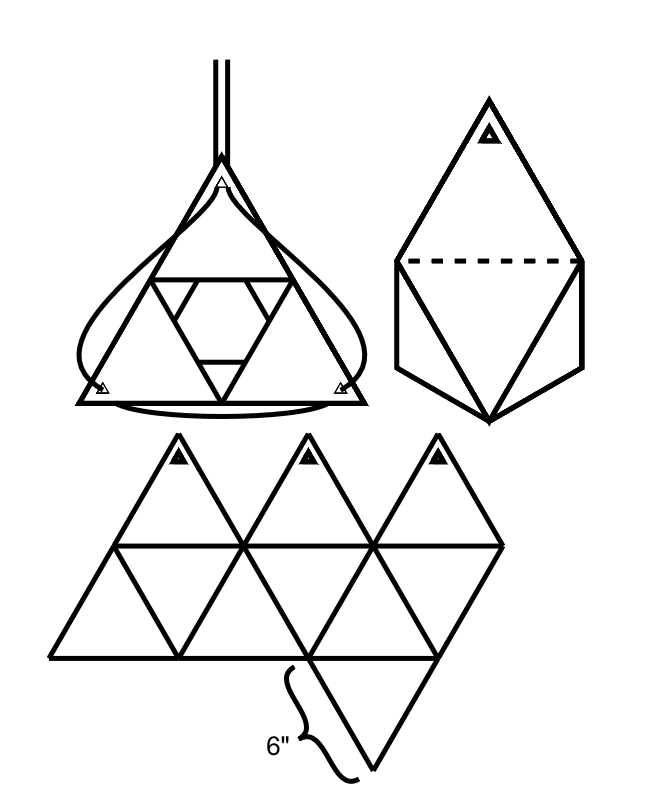
\includegraphics[width=4in]{imageset/uploadimages/artbox.png} The ArtBox is folded
up from 6 inch triangles as shown.

These shapes are all printed out on a laser cutter, cut out of
cardboard, or cut and laminated from paper, and then carried around in
the ArtBox along with a box cutter, sharpies of various colors, and a
pair of scissors. We start making all our cardboard things with making
this thing and teaching other to replicate it.

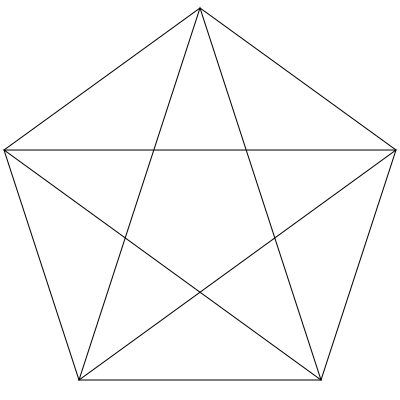
\includegraphics[width=4in]{imageset/uploadimages/pentagram.png} A fractal
pentagram colored in.

The pentagram and pentagon are beautiful, and very distinct when drawn
with tools versus freehand. A cardboard sign with a fractal pentagram
colored in with colored markers is a powerful self-replicating symbol
which can be used to spread our memes in the world. We use it to spread
our system initially just spreading the domain which points to the main
Pibrary of Trash Robot at www.trashrobot.org. These can be made in large
numbers with cardboard trash we find on the street or in dumpsters, and
can be placed in public spaces as part of our complex mixed reality
social media for gaming and community building. These are also boards on
which we can place the pieces discussed in the Icon Magic chapter.

\includegraphics[width=4in]{imageset/uploadimages/hexagram.png} A hexagram colored
in.

The hexagram is another beautiful and simple shape which can be drawn
easily with our tool set but which is hard to draw well freehand. Again,
this is used as an open brand, a sign to draw people in and promote our
network, and a generic board for placing other symbols.

\includegraphics[width=4in]{imageset/uploadimages/hexboard.png} The hex board is a
generic game board which can be used for placing generic icon pieces as
documented in the next chapter. This can be used as a space for
generalized organization of thought. Construct with the equilateral
triangle.

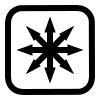
\includegraphics[width=4in]{imageset/uploadimages/chaos.png} The eight arrows of
chaos represents the idea of self-replication in the abstract. This is
the symbol on the cover of this book, and when combined with the
replicated and rotated pairs of two circles represents Geometron Magic,
this book and its contents.

\includegraphics[width=4in]{imageset/uploadimages/chaosconstruction.png} The
construction of the Geometron Magic symbol. Each circle has diameter of
three inches. Centers of circles are all 3/4 inches out from center.
Arrows are drawn with the Golden Triangle. Use a compass, an optional
tool of the ArtBox, or a drink lid and create a shape set to match its
size.

We also use Action Geometry to make textile crafts, including wearable
crafts like shirts and pants and hats which also form self-replicating
media, as they are constructed with the tools of Action Geometry and cut
out of trash clothing, making lines of clothing which are themselves
self-replicating media made out of trash.

Making self-replicating geometric art on cardboard is also a soothing
ritual, a form of art anyone can do anytime anywhere for any purpose.
The creation of a ritual like this helps to spread our culture and
civilization. Many geometric constructions on cardboard spreading along
the streets of the world form a global-sized game board on which game
tokens can be placed. These tokens will be discussed in the Icon Magic
chapter. Complex networks of interlinked maps and text documents
integrate the physical street and its media with our digital
self-replicating media. The Path of Geometron, described in a later
chapter, tells how we will build these Street Books using the Map Book
format, on our Geometron Magic book tour.
